\section{Sparse Reconstruction}

In this section, we implement various algorithms
to generate a sparse reconstruction of a scene
from two sample images, using two images of a
temple as a reference.

\subsection{Eight Point Algorithm}

\begin{enumarabic}
  \item Recovered Fundamental Matrix:
    \[
      F = \bmat{
        -1.12822743 \times 10^{-9} & 1.23273153 \times 10^{-7} & -6.24786160 \times 10^{-6} \\
        6.41080466 \times 10^{-8} & 1.04807659 \times 10^{-10} & -1.11138892 \times 10^{-3} \\
        -1.31615524 \times 10^{-5} & 1.06851400 \times 10^{-3} & 4.47839257 \times 10^{-3}
      } \qquad \text{(see Figure \ref{fig:raw-f} for raw matrix)}
    \]

    \item Epipolar Line Visualizations:
      \begin{figure}[H]
        \centering
        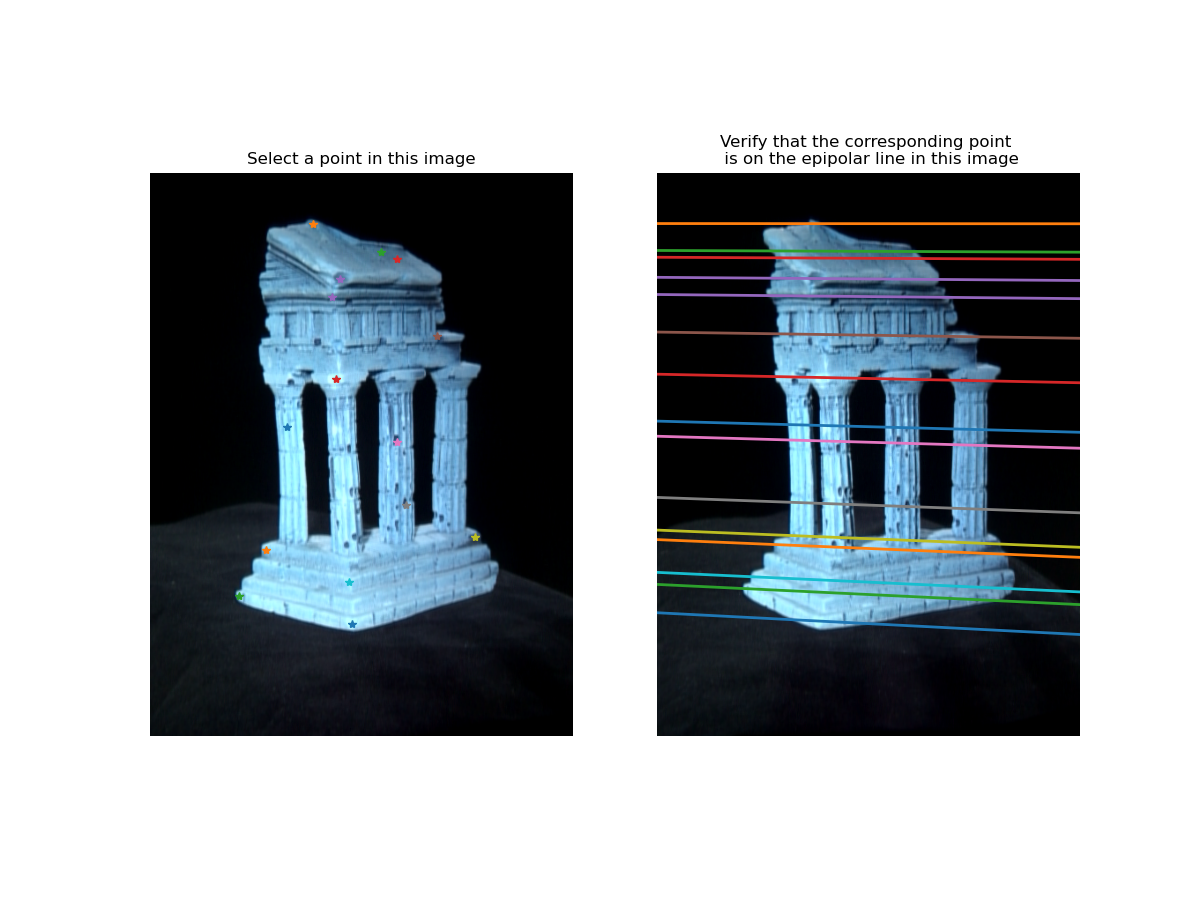
\includegraphics[width=\textwidth]{./figures/epipolar-lines.png}
        \caption{Epipolar lines}
      \end{figure}
\end{enumarabic}

\newpage
\subsection{Epipolar Correspondences}

\begin{enumarabic}
  \item Epipolar Correspondences \\
    To measure similarity, I used a window around each two points being compared,
    one from the first image and one from the second image.
    I then computed the sum of squared differences (SSD) between the two windows
    and used this as a measure of similarity.
    I experimented with different window sizes; size $5$ did not seem to
    work well especially for non-corner points.
    Size $20$ worked admissibly well although, as demonstrated below,
    still fails for points that are entirely in the dark background.

    \begin{figure}[H]
      \centering
      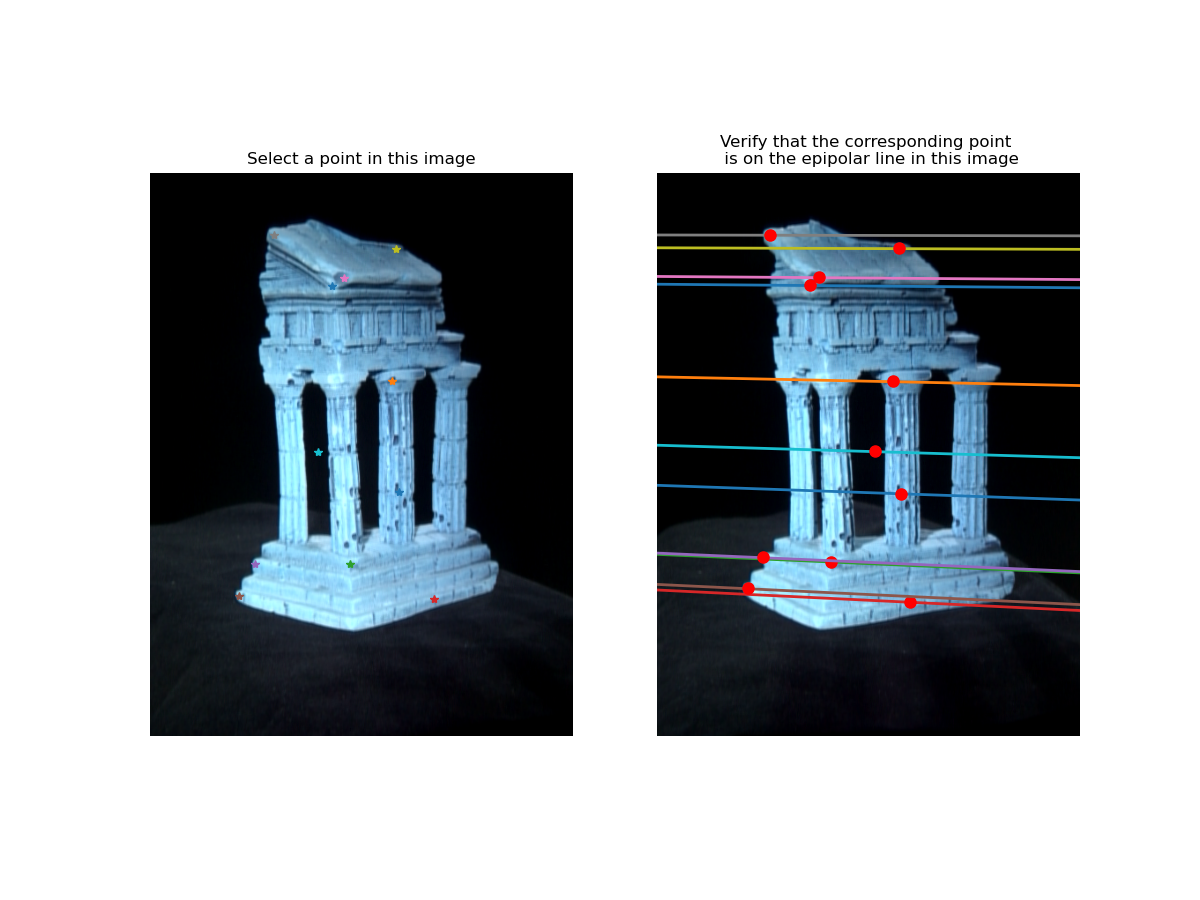
\includegraphics[width=\textwidth]{./figures/epipolar-correspondences.png}
      \caption{Epipolar lines}
    \end{figure}

  \newpage
  \item Failure Cases \\
    The matching algorithm fails when there aren't enough unique features
    to distinguish a point from other points on the same epipolar line.
    A simple example is clicking in the black region in the image.
    A more interesting example is the point on the red line,
    which gets mismatched to a wrong point on the epipolar line.
    One potential solution can be to make the window larger,
    but that eventually makes the algorithm slower.
    Maybe combining that with some dynamic programming
    (instead of recomputing the window every time, maintain the
    sliding values and only update the edges of the window when
    moving to the next point on the epipolar line).

    \begin{figure}[H]
      \centering
      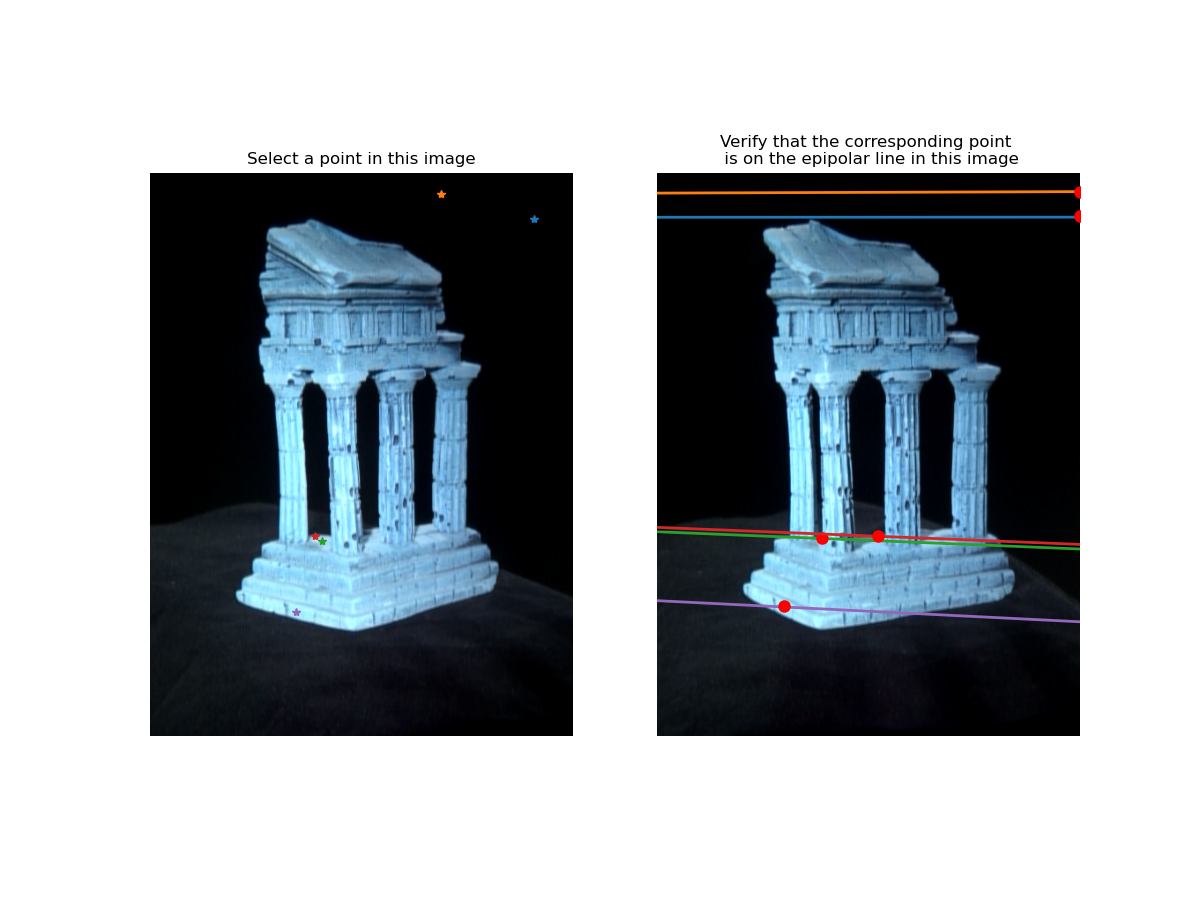
\includegraphics[width=\textwidth]{./figures/correspondence-fails.png}
      \caption{Failure case}
    \end{figure}
\end{enumarabic}

\subsection{Essential Matrix}

\begin{enumarabic}
  \item Recovered Essential Matrix
    \[
      E = \bmat{
        -4.90914507 \times 10^{-1} & 3.96179658 & 2.19734674 \\
        2.12129669 & -1.48056692 \times 10^{-1} & -9.42668155 \\
        6.10057409 \times 10^{-2} & 9.54224292 & 1.09934587 \times 10^{-1}
      } \qquad \text{(see Figure \ref{fig:raw-e} for raw matrix)}
    \]
\end{enumarabic}

\newpage
\subsection{Triangulation}

\begin{enumarabic}
  \item Determining The Correct P-Matrix \\
    As mentioned in the hint, the correct configuration of the P-matrix
    should have the most points in front of the camera.

    % algorithm
    \begin{center}
      \begin{minipage}{.6\textwidth}
        \begin{answer}
          \begin{algorithm}[H]
            % count_invalid
            \caption{Counting Invalid Points}
            \begin{algorithmic}[1]
              \Function{count\_invalid}{$X[1..n]$}
                \State $c \gets 0$
                \For {$i \gets 1 \text{ to } n$}
                  \If {$X[i][3] < 0$}
                    \State $c \gets c + 1$
                  \EndIf
                \EndFor
                \State \Return $c$
              \EndFunction
            \end{algorithmic}
          \end{algorithm}
          \begin{algorithm}[H]
            \caption{Determining the Correct P-Matrix}
            \begin{algorithmic}[1]
              \State $P_2[1\ ..\ 4] \gets \mathbf{camera2}(E)$
              \For {$i \gets 1 \text{ to } 4$}
                \State $X_i \gets \textsc{triangulate}(P_1, \text{points}_1, P_2[i], \text{points}_2)$
                \State $A[i] \gets \textsc{count\_invalid}(X_i)$
              \EndFor
              \State \Return $P_2[\mathbf{argmin}(A)]$
            \end{algorithmic}
          \end{algorithm}
        \end{answer}
      \end{minipage}
    \end{center}

  \step
  \item Reprojection Error
    \[ 
      \text{Points$_1$ Reprojection Error} = 0.8521671561856665
    \]
    \[
      \text{Points$_2$ Reprojection Error} = 0.8630693907867739
    \]
  % invalid_count = [65, 223, 0, 288]
  % PTS1 ERROR: 0.8521671561856665
  % PTS2 ERROR: 0.8630693907867739
    
\end{enumarabic}

\newpage
\subsection{Test Script}

\step
Examples of generated sparse reconstructions are shown below.

\begin{figure}[H]
  % minipages
  \centering
  \begin{minipage}{.49\textwidth}
    \centering
    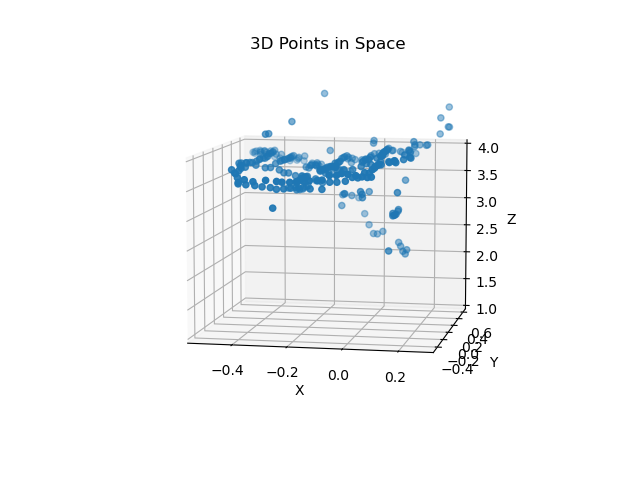
\includegraphics[width=\textwidth]{./figures/sparse-1.png}
    \caption*{Perspective 1}
  \end{minipage}
  \hfill
  \begin{minipage}{.49\textwidth}
    \centering
    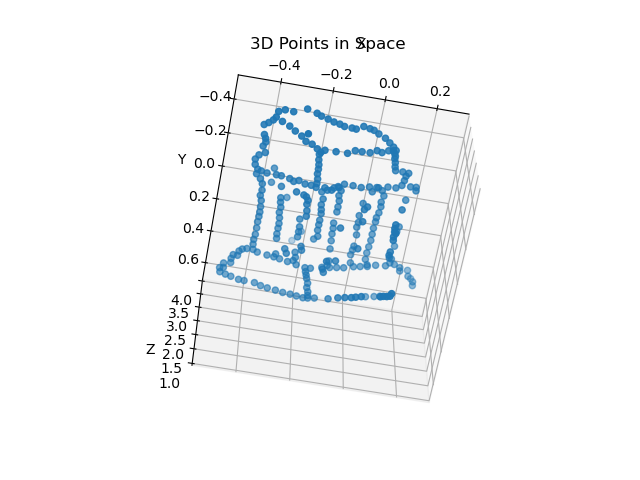
\includegraphics[width=\textwidth]{./figures/sparse-2.png}
    \caption*{Perspective 2}
  \end{minipage}
  \hfill
  \begin{minipage}{.49\textwidth}
    \centering
    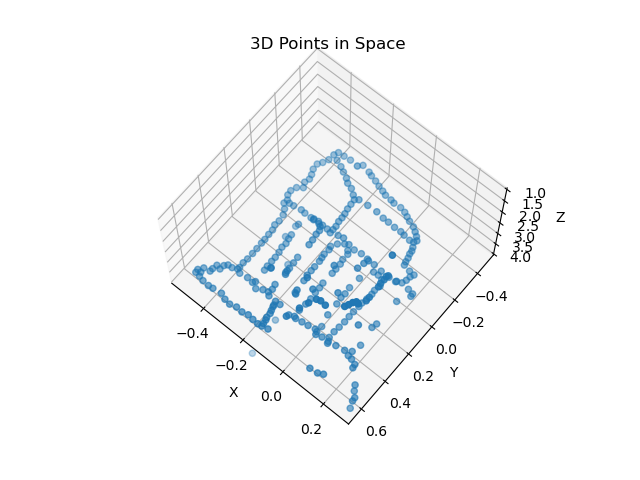
\includegraphics[width=\textwidth]{./figures/sparse-3.png}
    \caption*{Perspective 3}
  \end{minipage}
\end{figure}
